diff --git a/reorder_main_text.tex b/../../../manuscript/reorder_main_text.tex
index 858fe9b..1cb25e3 100644
--- a/reorder_main_text.tex
+++ b/../../../manuscript/reorder_main_text.tex
@@ -379,21 +379,22 @@ Motif participation describes extinction risk
         Participation in the three-species chain motif showed the opposite trends.
     
 
-        Digging deeper and exploring how persistence varied with the proportion of a motif in the species' participation vector, disturbance, and overall network structure (size and connectance), we found that the relationship between the proportion of omnivory in the participation vector and probability of persistence depended strongly on the connectance of the network.
+        In depth exploration of how persistence varied with the proportion of a motif in the species' participation vector, disturbance, and overall network structure (size and connectance), showed that the relationship between the proportion of omnivory in the participation vector and probability of persistence depended strongly on the connectance of the network Fig.~\ref{Fig 2}.
         Higher proportions of omnivory were associated with lower probabilities of persistence when connectance was low, regardless of network size or strength of disturbance.
         At moderate connectance, however, higher proportions of omnivory were associated with greater probabilities of persistence when disturbance was weak.
-        In the most-connected networks, higher proportions of omnivory were associated with greater probabilities of persistence at all levels of disturbance.
+        In the most-connected networks, higher proportions of omnivory were associated with greater probabilities of persistence at all levels of disturbance. 
 
-        The relationships between other motifs and persistence were more consistent over different levels of connectance and network size.
-        Slopes of the motif proportion-persistence relationships for the apparent competition and direct competition motifs were steepest in large and less-connected networks but the directions of slopes varied only with the strength of disturbance, as in Fig.~\ref{Fig 2}.
+        The relationships between the proportion of other motifs and persistence were more consistent over different levels of connectance and network size.
+        Slopes of the motif proportion-persistence relationships for the apparent competition and direct competition motifs were steepest in large and less-connected networks, but the directions of slopes varied only with the strength of disturbance, as in Fig.~\ref{Fig 2}.
         The relationship between proportion of the three-species chain in the participation vector and persistence was very similar across all levels of size and connectance.
 
+         The effects of network size were overall limited Fig.~\ref{Fig 2}.
         
         Considering each network separately ....
         
 
-
-    \subsection*{Species persistence and other network properties}
+% Total frequencies of motifs in the whole network
+    \subsection*{Species persistence and network motif profile}
 
         As well as the frequency with which each species appears in each motif, we can use the total frequencies of each motif in the whole network (i.e., the network's motif profile) to describe its structure.
         The average probability of persistence of all consumers in the network varied with the frequencies of different motifs in this profile.
@@ -544,7 +545,7 @@ Motif participation describes extinction risk
 
 \section*{Figures}
     
-
+        % FIGURE 1
         \begin{figure}[hb!]
         \centering
         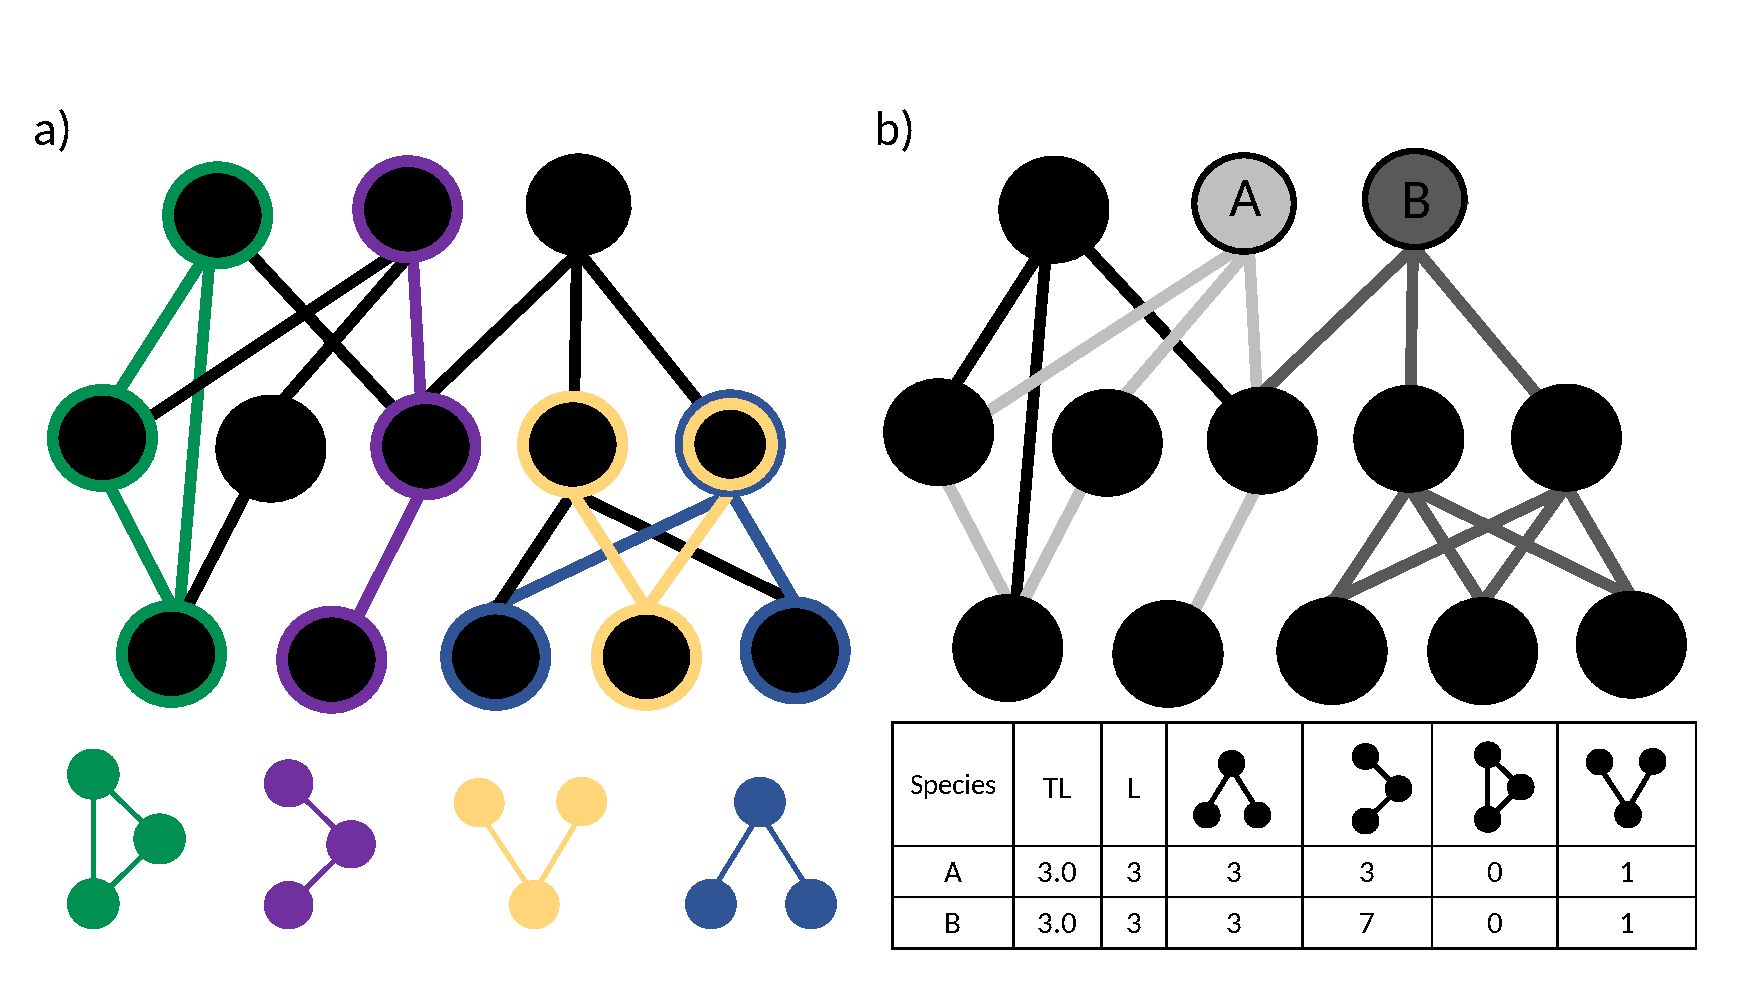
\includegraphics[width=1.0\textwidth]{figures/concept_fig_ver2.eps}
@@ -554,7 +555,7 @@ Motif participation describes extinction risk
     \label{fig:concept}
     \end{figure}
 
-    
+        % FIGURE 2
         \begin{figure}[hb!]
         \centering
         \includegraphics[width=0.85\textwidth]{figures/persistence_motif_participation.eps}
@@ -562,7 +563,7 @@ Motif participation describes extinction risk
     \label{fig:prop_lmer_all}
     \end{figure}
         
-
+        % FIGURE 3
     \begin{figure}[hb!]
         \centering
         \includegraphics[width=\textwidth]{figures/roles_vs_TL.eps}
@@ -571,6 +572,7 @@ Motif participation describes extinction risk
         \label{fig:motifs_vs_TL_and_deg}
     \end{figure}        
 
+        % FIGURE 4
     \begin{figure}[ht!]
         \centering
         \includegraphics[width=\textwidth]{figures/persistence_vs_SC_lm.eps}
@@ -590,10 +592,10 @@ Motif participation describes extinction risk
     %     \label{fig:roles_vs_SC}
     % \end{figure}
 
-
+    % FIGURE 5
     \begin{figure}[hb!]
     \centering
-        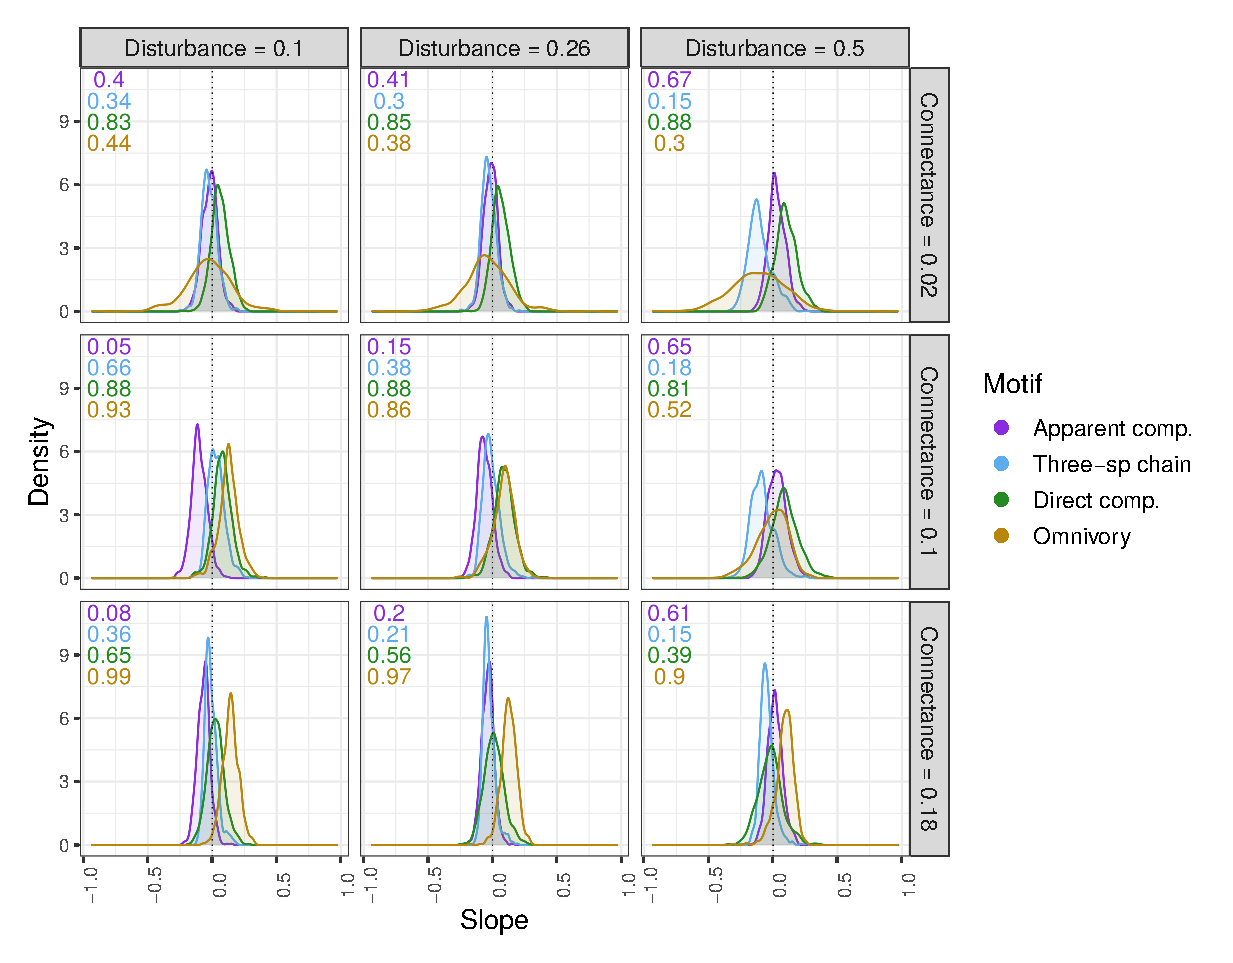
\includegraphics[width=\textwidth]{figures/prop_dens_bp_vs_C_allS.eps}
+        \includegraphics[width=\textwidth]{manuscript/figures/Fig4.pdf}
         \caption{Here we show the density (y-axis) of slopes (x-axis) of persistence against proportion of different motifs for all simulated webs of all sizes - a visualization of how an increased proportion of each motif (different colored lines) affects persistence of consumer species. Columns show the result for various disturbances on the basal level, from $\pi_{disturbed} = 0.1$ (left) to $\pi_{disturbed} = 0.5$ (right). Rows show various levels of connectance. The dotted, vertical lines indicate zero on the x-axis. A negative slope value reflects a negative relationship between increased participation in a motif and persistence, while a positive slope value reflects a positive relationship - an increased proportion of a specific motif increases persistence. The fraction of replicates with a slope greater than zero are stated in numbers in each sub-plot, the color corresponding to each motif (legend). }
         \label{fig:density_prop_C}
     \end{figure}    
